% Vygenerováno skriptem vysledky.py. Vyžaduje \usepackage{graphicx} v preambuli.

\begin{figure}[htbp]
\centering
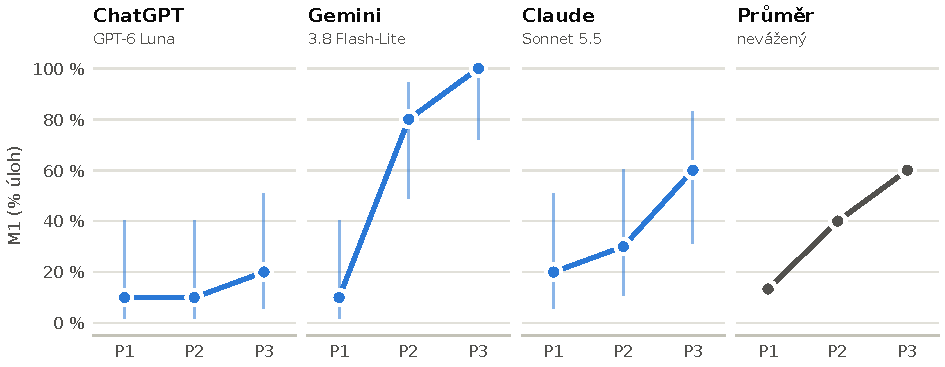
\includegraphics[width=\linewidth]{vystupy/graf_m1.pdf}
\caption{M1 podle systému a~podmínky promptu na testovací sadě. Body jsou podíly úloh s~úplnou a~přesnou množinou podob, svislé úsečky 95\% Wilsonovy intervaly. Průměr systémů je nevážený a~bez intervalu.}
\label{fig:m1}
\end{figure}

\begin{figure}[htbp]
\centering
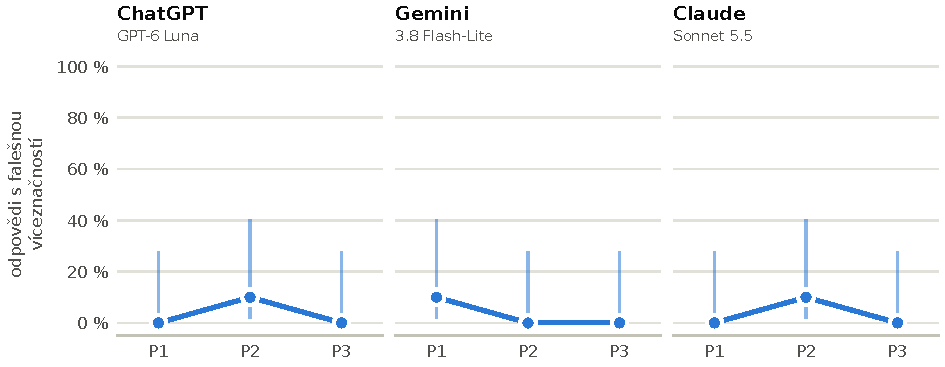
\includegraphics[width=\linewidth]{vystupy/graf_falesne.pdf}
\caption{Podíl odpovědí, v~nichž systém označil za víceznačné slovo, které víceznačné není, s~95\% Wilsonovými intervaly. Odpovědi vyřazené pro chybu formátu se sem nepromítají.}
\label{fig:falesne}
\end{figure}

\begin{figure}[htbp]
\centering
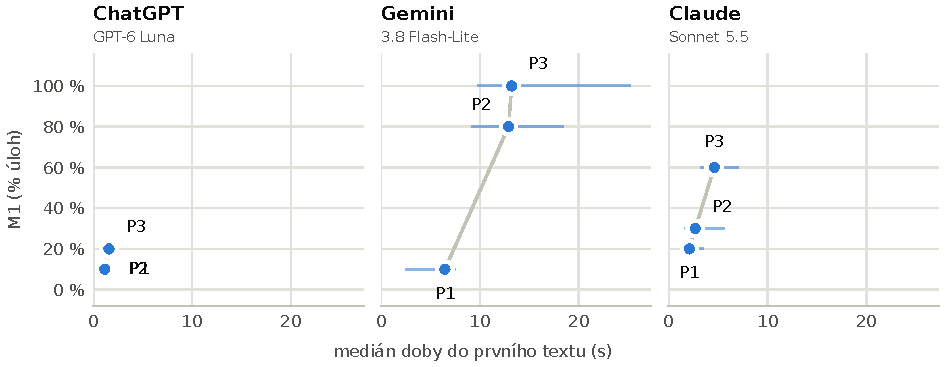
\includegraphics[width=\linewidth]{vystupy/graf_latence.pdf}
\caption{Kvalita a~rychlost: M1 proti mediánu doby do prvního textu odpovědi. Vodorovné úsečky jsou mezikvartilová rozpětí. Intervaly pro M1 jsou na obrázku~\ref{fig:m1}.}
\label{fig:latence}
\end{figure}
